% Chapter 1

\chapter{Introducere} % Write in your own chapter title
\label{Capitolul1}
\lhead{Capitolul 1. \emph{Introducere}} % Write in your own chapter title to set the page header

\section{Motiva\c{t}ie}

Dezvoltarea \c{s}i utilizarea sistemelor de m\u{a}surare programabile au fost explorate pe scar\u{a} larg\u{a}. Posibilitatea de a modifica procedura de m\u{a}surare prin simpla schimbare a algoritmului executat de un calculator f\u{a}r\u{a} a \^{i}nlocui componentele hardware face activitatea experimental\u{a} mai u\c{s}oara.

Timp de mul\c{t}i ani, instrumentele electronice au fost u\c{s}or de identificat. De\c{s}i variaz\u{a} \^{i}n m\u{a}rime \c{s}i func\c{t}ionalitate, toate sunt sub forma unei cutii, av\^{a}nd un panou frontal \c{s}i un display. Acestea sunt foarte puternice \c{s}i sunt concepute pentru a executa una sau mai multe sarcini men\c{t}ionate de c\u{a}tre v\^{a}nz\u{a}tor.

Cu toate acestea, utilizatorul nu le poate extinde sau particulariza. Butoanele, circuitele interne \c{s}i func\c{t}iile disponibile utilizatorului sunt speficice naturii instrumentului. Adoptarea pe scar\u{a} larg\u{a} a PC-ului \^{i}n ultimii dou\u{a}zeci de ani a dat na\c{s}tere unui nou mod de m\u{a}surare \c{s}i automatizare pentru ingineri.

Un prim model conceptual al instrumenta\c{t}iei bazat\u{a} pe calculator este prezentat \^{i}n figura de mai jos:

\begin{figure}[tbp]
  \centering
  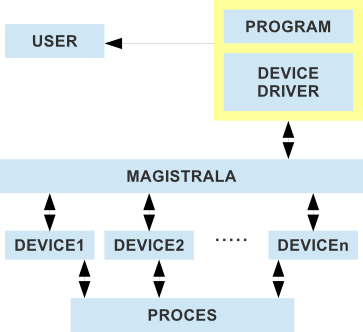
\epsfig{file=Figuri/model_instrumentatie.eps,width=0.5\linewidth,clip=}
  \caption{Model al instrumenta\c{t}iei bazate pe calculator}
  \label{figsistem}
\end{figure}

Un singur utilizator controleaz\u{a} sistemul. Exist\u{a} o singur\u{a} structur\u{a} de control, format\u{a} din utilizator \c{s}i programul care comand\u{a} instrumentele ata\c{s}ate magistralei.

Instrumentele sistemului pot folosi fie o comunica\c{t}ie serial\u{a}, bazat\u{a} pe standardul RS-232, fie o comunica\c{t}ie paralela, bazat\u{a} pe standardul GPIB.

Scopul \emph{Standard Commands for Programmable Instruments (SCPI)} este acela de a facilita reducerea timpului de dezvoltare pentru programele implementate \^{i}n sistemele de m\u{a}surare \c{s}i control precum \c{s}i de a permite schimbarea aparatelor (eventual produse de firme diferite) \^{i}n cadrul aceluia\c{s}i sistem de m\u{a}surare condus de calculator. Acest lucru se realizeaz\u{a} prin introducerea unor comenzi standardizate c\u{a}tre aparate \c{s}i a unor tipuri posibile de r\u{a}spuns al acestora. Spre exemplu, comanda:
\begin{center}
	\begin{verbatim}
	MEASURE:FREQ?
	\end{verbatim}
\end{center}

are aceea\c{s}i sintax\u{a} pentru toate aparatele de un anumit tip (de exemplu, multimetre) fabricate de diver\c{s}i producatori - consisten\c{t}\u{a} vertical\u{a} - dar \c{s}i pentru aparate cu func\c{t}ii diferite (de exemplu, osciloscoape, num\u{a}r\u{a}toare) - consisten\c{t}\u{a} orizontal\u{a}.

SCPI nu este un limbaj de programare (cum sunt, de exemplu, Pascal sau C), ci un limbaj de comenzi care define\c{s}te comenzile c\u{a}tre aparate, parametrii \c{s}i formatul acestora. SCPI furnizeaz\u{a} un \c{s}ir de caractere ASCII care vor fi transmise prin rutine specifice aparatelor unde vor fi, apoi, prelucrate prin intermediul limbajului TMSL (\emph{Hewlett-Packard's Test and Measurement System Language}).

SCPI s-a dezvoltat, \^{i}n principal, p\u{a}str\^{a}nd o compatibilitate cu norma IEEE-488 \c{s}i utiliz\^{a}nd formatul de date al acestei norme. Cu toate acestea, utilizarea SCPI nu este limitat\u{a} la interfa\c{t}a IEEE-488, comenzile acestuia put\^{a}nd fi transmise \c{s}i prin interfe\c{t}ele VXI sau RS-232 \c{s}i, \^{i}n plus, fiind continuu supus complet\u{a}rilor necesitate de dezvoltarea hardware-ului specific, \^{i}n urma recomand\u{a}rilor f\u{a}cute de un consor\c{t}iu de firme, alc\u{a}tuit din reprezentan\c{t}i ai leader-ilor pe pia\c{t}a instrumentelor de m\u{a}surare: Hewlett-Packard, Tektronix, Fluke (Philips), Keithley, Rohde\&Schwarz etc.

Cu toate c\u{a} SCPI define\c{s}te comenzile specifice aparatelor de m\u{a}surare "inteligente", nu sunt indicate nici un fel de date tehnice privind exactitatea, rezolu\c{t}ia, domeniul de m\u{a}surare ale acestora; astfel nu poate fi \^{i}n totalitate garantat\u{a} compatibilitatea aparatelor \^{i}n cadrul unui sistem comandat prin intermediul SCPI.

\section{Scop}

Aceast\u{a} lucrare \^{i}\c{s}i propune analizarea \c{s}i implementarea unei interfe\c{t}e SCPI de comand\u{a} pentru generatorul de semnal BK 4070. Din cauza faptului c\u{a} acest generator suport\u{a} un anumit set de comenzi \c{s}i comunica\c{t}ie serial\u{a}, prin standardul RS-232, s-a dorit integrarea acestuia \^{i}ntr-un sistem mai mare, compatibil cu standardul SCPI.

Se vor folosi aplica\c{t}iile Lex \c{s}i Yacc pentru generarea gramaticii \c{s}i sintaxei interfe\c{t}ei SCPI, urm\^{a}nd ca aplica\c{t}ia generat\u{a} s\u{a} trimit\u{a} serial comenzi c\u{a}tre generatorul de semnal.

\section{Rezumat}

Lucrarea este structurat\u{a} \^{i}n trei par\c{t}i. Prima parte \^{i}\c{s}i propune descrierea aspectelor teoretice ale standardului SCPI. Se vor prezenta structura comenzilor precum \c{s}i clasele \^{i}n care se incadreaz\u{a} acestea.

A doua parte \^{i}\c{s}i propune prezentarea utilitarelor Lex \c{s}i Yacc. Vor fi descrise regulile pentru scrierea fi\c{s}ierelor, modul de execu\c{t}ie pentru generarea unui translator.

\^{I}n final, a treia parte \c{s}i cea mai important\u{a}, prezint\u{a} implementarea \c{s}i func\c{t}ionarea interfe\c{t}ei SCPI de comand\u{a} pentru un generator de semnal.
